\PassOptionsToPackage{numbers,sort&compress}{natbib}
\documentclass[preprint,numbers,a4paper]{elsarticle}
\usepackage[T1]{fontenc}
\usepackage[utf8]{inputenc}
\usepackage{amsmath,amssymb,amsthm,bm,booktabs,graphicx,siunitx}
\usepackage[margin=2cm]{geometry}
\usepackage{hyperref}

\newtheorem{theorem}{Consistency criterion}
\newtheorem{lemma}{Lemma}
\graphicspath{{figures/}}
\usepackage{xr-hyper}
%\linenumbers
\externaldocument{02_track_D_chaos_SI}
\usepackage[nameinlink,capitalize,noabbrev]{cleveref}
\usepackage[expansion=false]{microtype}
% Cross-references to the Supplement (e.g.\ \cref{SI-tab:anchor-gap})
% print with its S-numbering (e.g.\ Table S10), set by the SI counters.
\sisetup{mode = match}
\newcommand{\dd}{\,\mathrm{d}}
\newcommand{\Tr}{\operatorname{Tr}}

% Prevent all line breaks in inline equations.
\binoppenalty=10000
\relpenalty=10000

\hypersetup{
    colorlinks,
    linkcolor={blue!50!black},
    citecolor={blue!50!black},
    urlcolor={blue!80!black}
}

\setlength{\emergencystretch}{1.5em}
\bibliographystyle{elsarticle-num}
\begin{document}

\begin{frontmatter}

\title{Synthetic-flux control of hyperchaos order in a dissipative optomechanical model}

\author[inst1]{Stella Rolande Mbokop Tchounda}
\author[inst1]{Carolle Tchodimou}
\author[inst2]{Philippe Djorwe}
\author[inst3]{Sifeu Takougang Kingni}
\author[inst1,corref]{Serge Guy Nana Engo}

\ead{serge.nana-engo@facsciences-uy1.cm}
\cortext[corref]{Corresponding author}

\affiliation[inst1]{organization={Department of Physics, Faculty of Science, University of Yaound\'e I}, city={Yaound\'e}, country={Cameroon}}
\affiliation[inst2]{organization={Department of Physics, Faculty of Science, University of Ngaound\'er\'e}, city={Ngaound\'er\'e}, country={Cameroon}}
\affiliation[inst3]{organization={Department of Mechanical, Petroleum and Gas Engineering, National Advanced School of Mines and Petroleum Industries, University of Maroua}, city={Maroua}, country={Cameroon}}

\begin{abstract}
Within a normalized six-dimensional model of dissipative optomechanics (one cavity and two mechanical resonators), the synthetic-flux phase $\Phi_{\rm syn}$ provides open-loop selection of the \emph{order} of a drive- and coupling-gated hyperchaos transition---up to four simultaneously positive Lyapunov exponents, exceeding reported single-mode optomechanical benchmarks. The route is drive-gated: a Neimark--Sacker onset at $E^{*}=\num{1.060}$ ($\theta=0$) and $E^{*}=\num{0.975}$ ($\theta=\pi/2$), re-stabilization at the sampled intermediate drive ($E=\num{2.0}$, count near zero), and finite-time positive-exponent counts reaching three at $E=\num{4.0}$ and four at $E=\num{8.0}$. A phase-consistent Floquet--Lyapunov protocol (monodromy multipliers, dissipative volume balance $\sum\lambda_i=\operatorname{Tr}(J)=-1.04$, and a \num{432}-run classification ensemble spanning twelve seeds, twelve phases, and three drives) supports the classification under the stated protocol, and orbit continuation localizes the onset. As a secondary model-level clarification, the matched-resource force-sensing protocol returns a null gain on the chaotic attractor (flux-on Fisher information $\num{0.54}\times$ flux-off at the resolved $E=\num{4}$ points) and only a modest order-unity gain ($\num{1.039}\pm\num{0.014}$) on the stable orbit, consistent with the matched-Fisher lemma. Truncated-Fock and truncated-Wigner checks support the mean-field description at selected points. All results are strictly model-level---the sector lies $\num{2542}\times$ beyond anchored silicon couplings, and closing that gap requires ultrasonic characterization of the mechanical degeneracy $\omega_2$, a measured inter-resonator hopping $J_m$, and a genuine gigahertz platform.
\end{abstract}

\begin{keyword}
hyperchaos \sep Lyapunov spectrum \sep Bifurcation control \sep Dissipative optomechanics \sep Synthetic gauge flux \sep Neimark--Sacker bifurcation
\end{keyword}

\end{frontmatter}



\section{Introduction}

The order of a hyperchaos transition---the number of simultaneously
positive Lyapunov exponents---has so far been limited to two in
single-mode quadratic optomechanical platforms
\cite{HalefShomroni2025}. Whether a synthetic-flux phase can raise
that order in a multi-mode radiation-pressure model, and whether the
resulting geometric control can be corroborated by full-spectrum methods,
had not been resolved. Hyperchaos order quantifies the
dimensionality of the unstable manifold and therefore the number of
independent directions along which small perturbations grow. Selecting
a desired dynamical regime by tuning a control parameter is a classic
theme in nonlinear dynamics \cite{ott1990,boccaletti2000}.

We show, within one normalized six-dimensional model (building on the
topology of Muthukumar \emph{et~al.}~\cite{muthukumar2025doi}), that the synthetic-flux phase $\Phi_{\rm syn}$ reproducibly controls the \emph{order} of a drive- and
coupling-gated hyperchaos route---up to four simultaneously unstable
directions, beyond reported single-mode optomechanical benchmarks. The onset is
localized to a Neimark--Sacker bifurcation and is corroborated by a
phase-consistent Floquet--Lyapunov protocol. The route itself is
structured rather than monotonic: after the torus onset the orbit
nearly re-stabilizes in a window at intermediate drive, and the
positive-exponent count then climbs through three up to four as the
drive increases. As a secondary geometric
clarification, the same matched measurement on the chaotic attractor
yields no flux-induced sensing enhancement. These are strictly
model-level results: the strong-coupling sector explored here lies far
beyond present experimental anchors. A nonlinear optomechanical platform
provides the physical substrate: radiation-pressure nonlinearity,
coherent mechanical motion, dissipation, periodic modulation, and a
complex hopping amplitude that supports a synthetic gauge structure
\cite{aspelmeyer2014,kippenberg2008,marquardt2006,carmon2007,alphonse2022},
together with Floquet engineering
\cite{oka2009,goldman2014,bukov2015,kitagawa2010,peano2015,sanavio2020}.

The central result is shown in \cref{fig:hyperchaos-map}: the synthetic-flux phase $\Phi_{\rm syn}$ selects
the number of simultaneously positive Lyapunov directions in the
strongly damped, strongly coupled sector: the count reaches
four at $E=\num{8}$, $\theta=-\pi/2$ (seed-dependent; see below), and drops to two at
$\theta=0\pmod{\pi}$. Relative to prior work, Muthukumar \emph{et al.}~\cite{muthukumar2025doi}
established the one-cavity/two-resonator topology and reported
phase-selected chaotic regimes at resolved-sideband couplings
\cite{mondal2024doi,Xu2025}, but did not resolve the \emph{full Lyapunov
spectrum} (so that the instability order cannot be counted) nor
quantify a flux-dependent advantage under matched resources. Chaos in
optomechanical models is established in single-mode and hybrid
configurations \cite{larson2011,wang2016,chen2024}, and hyperchaos has
been generated in other driven nonlinear platforms such as
delayed-feedback semiconductor lasers \cite{vicente2005}.
The closest full-spectrum report \cite{HalefShomroni2025} is
restricted to quadratic single-mode coupling where no
synthetic-flux phase is available. We extend the Muthukumar
topology by making the convention $\Delta=-\Delta_{\mathrm M}$
explicit, allowing $g_1\neq g_2$, and scanning the strongly
damped, strongly coupled sector where the full spectrum resolves up
to four simultaneously unstable directions. A second full map at reduced
coupling ($g_1/\omega_m=\num{0.2}$) shows the same flux modulation with a
lowered ceiling (see Results). We further replace the
qualitative sensing proposal by a matched-resource
measurement-Fisher protocol
\cite{braunstein1994,purdy2017,teufel2011,gavartin2012,li2021a},
applied both on the weakly coupled reference orbit and on the
chaotic attractor.

We address three operational questions at the model level. First, does
$\Phi_{\rm syn}$ control the order of a drive- and coupling-gated
hyperchaos \cite{rossler1979}, with the route localized by a
continued-orbit scan
\cite{kuznetsov2004,guckenheimer1983,strogatz2015} to a Neimark--Sacker
bifurcation? Second, do monodromy multipliers and the long-time Lyapunov
spectrum \cite{benettin1980,wolf1985,eckmann1985} agree on the same periodic
orbit, thereby validating the
transition? Third (secondary), after thermal, vacuum and detector noise
are included, does a matched-resource measurement statistic retain a
flux-dependent signature on the stable orbit or on the chaotic
attractor? A positive answer to the first two questions constitutes the
central claim of this work---synthetic-flux control of hyperchaos order.
The null answer to the third supplies a geometric bound (matched-Fisher
lemma) showing that additional unstable directions do not automatically
yield metrological gain. Both results are to be read as normalized,
model-level demonstrations rather than device predictions.

\section{Model and conventions}

The one-cavity, two-mechanical-resonator topology and phase-dependent
hopping are due to Muthukumar \emph{et al.}~\cite{muthukumar2025doi};
the rotating-frame Hamiltonian used here is
\begin{equation}
\frac{H}{\hbar}=-\Delta a^\dagger a
+\sum_{j=1}^{2}\omega_j b_j^\dagger b_j
-\sum_{j=1}^{2}g_j a^\dagger a(b_j+b_j^\dagger)
+J\!\left(e^{i\theta}b_1^\dagger b_2+e^{-i\theta}b_2^\dagger b_1\right)
+i(Ea^\dagger-E^*a),
\label{eq:hamiltonian}
\end{equation}
with cavity mode $a$ and mechanical modes $b_j$. We use
$\Delta=\omega_c-\omega_L$ (so $\Delta=-\Delta_{\mathrm M}$ of
Ref.~\cite{muthukumar2025doi}, which takes the opposite sign), quadratures
$[X,Y]=i$, and the drive $E=\sqrt{\kappa}\,\alpha^{\rm in}$ in the shared
normalization. The present analysis allows $g_1\neq g_2$ and scans
the strongly damped, strongly coupled sector
$\kappa\sim\gamma\sim g\sim\num{1e-2}$--$\num{1}\,\omega_m$ in which the
hyperchaotic attractor is resolved. \textbf{A side-by-side comparison
with Ref.~\cite{muthukumar2025doi} is given in
\Cref{SI-tab:muthukumar-comparison}}.

The semiclassical factorization gives
\begin{align}
\dot\alpha &= \left(i\Delta-\frac{\kappa}{2}\right)\alpha
+i\sum_jg_j(\beta_j+\beta_j^*)\alpha+E(t),\\
\dot\beta_1 &= -\left(i\omega_1+\frac{\gamma_1}{2}\right)\beta_1
+ig_1|\alpha|^2-iJe^{i\theta}\beta_2,\\
\dot\beta_2 &= -\left(i\omega_2+\frac{\gamma_2}{2}\right)\beta_2
+ig_2|\alpha|^2-iJe^{-i\theta}\beta_1,
\label{eq:complex-eom}
\end{align}
with the real state $x=(\alpha_r,\alpha_i,\beta_{1r},\beta_{1i},\beta_{2r},\beta_{2i})^T$.
The hopping amplitude is written $J$ in the Hamiltonian and, identically,
$J_m$ in normalized ratios ($J_m\equiv J$).

For the three-link loop, the phase coordinate used in the analysis is the
gauge-invariant phase
\begin{equation}
\Phi_{\mathrm{syn}}=\arg(g_1Jg_2^*)\pmod{2\pi}.
\label{eq:flux}
\end{equation}
A redefinition of the mode phases may redistribute link phases but cannot change
$\Phi_{\mathrm{syn}}$. In the phase convention of \cref{eq:hamiltonian}
(all phase on the inter-resonator hopping, $g_1,g_2\in\mathbb{R}$) the
invariant reduces to the hopping phase, $\Phi_{\mathrm{syn}}\equiv\theta
\pmod{2\pi}$, so the two notations coincide and are used interchangeably in the
results; the invariant form is retained because it is the coordinate that
survives such a redefinition.

\section{Methods}

The numerical protocol is organized around three independent
consistency layers that must agree before any claim of hyperchaos
order is accepted. (i)~A drive-locked periodic orbit
is located as a fixed point of the one-period Poincaré map; its
linear stability is diagnosed by the monodromy matrix (Floquet
multipliers). (ii)~The same orbit is integrated with QR
reorthonormalization to obtain the full six-exponent Lyapunov
spectrum; positivity is accepted only when the spectrum, the
multipliers and the analytic dissipative trace (\cref{eq:trace})
are mutually consistent. (iii)~As a secondary geometric check, a matched-resource classical Fisher
information is evaluated on both the stable reference orbit and on
sampled trajectories of the chaotic attractor, under identical
noise and resource assumptions. All three layers are implemented with the same phase convention for
$\Phi_{\rm syn}$ (Eq.~\eqref{eq:flux}). Thresholds used to count
positive exponents ($\num{1e-4}$ weak, $\num{1e-3}$ strong) and the
precise definition of the matched Fisher protocol are stated once here
and used uniformly thereafter. The strong threshold $\num{1e-3}$ is chosen to lie above the scale of the mechanical damping rates ($\gamma/2\sim\num{0.01}$) while remaining larger than typical QR residuals on the stable reference grid; sensitivity of the integer count $n_+$ to displacements of this cut by factors of three to five is quantified in the Supplementary Material.

\subsection{Phase-augmented dynamics and implementation}

For a periodic drive with phase $\phi$ we write
\begin{equation}
\dot{x}=f(x,\phi;p),\qquad \dot\phi=\Omega,
\label{eq:augmented}
\end{equation}
with the augmented Jacobian $J_{\mathrm{aug}}=(\partial_x f,\partial_\phi f;0,0)$.
The analytic Jacobian $J=\partial f/\partial x$ is compared column by column
with central finite differences; the implemented dissipative trace
\begin{equation}
\Tr J=-\kappa-\gamma_1-\gamma_2,
\label{eq:trace}
\end{equation}
is an independent implementation check. One-period integrations use DOP853
\cite{dormand1980} with relative and absolute tolerances \num{1e-9} and \num{1e-11} (max step
$T/200$); drive-locked orbits are located by fixed-point iteration of the
one-period map to a residual below \num{1e-8}, and the monodromy is obtained
by simultaneous integration of the variational equations.

\subsection{Periodic orbit and Floquet analysis}

A drive-locked periodic orbit is obtained from the fixed point of the
one-period Poincar\'e map; around it the fundamental matrix satisfies
\begin{equation}
\dot{\Phi}(t)=A(t)\Phi(t),\;\Phi(0)=\mathbb{I},\;M(T)=\Phi(T),
\label{eq:monodromy}
\end{equation}
with Floquet rates $\rho_i=T^{-1}\log|\mu_i|$. The same orbit is
integrated with QR/Benettin reorthonormalization
\cite{shimada1979,benettin1980,wolf1985,eckmann1985} to obtain the full Lyapunov
spectrum; a positive exponent is accepted only after agreement with
the multipliers, the divergence given by \eqref{eq:trace}, and the
bounded-attractor diagnostics. In the full-spectrum classification an exponent is
counted as positive only above the thresholds stated at the start of
this section (\Cref{SI-tab:si-threshold-sensitivity}) whereas
the Kaplan--Yorke sum uses strictly positive exponents; the threshold
count and the Kaplan--Yorke sum can differ near zero. The Lyapunov QR uses a fixed-step fourth-order Runge--Kutta (RK4)
($\num{1e-2}$ step, QR every ten steps), discarding a $\num{1e5}$
transient and integrating $\num{1e6}$ steps per trajectory for the
production spectra, and $\num{2e5}$ and $\num{2e6}$ steps for the
Floquet--Lyapunov consistency validation of \cref{sec:results}. The theorem
bounds are established at $\num{2e6}$ steps while production spectra use
$\num{1e6}$ steps, additionally supported by the six-point
window-convergence probe (\Cref{SI-tab:si-convergence-v2}). Orbit
location uses adaptive DOP853 and long QR spectra use fixed-step RK4; the
quoted Floquet--QR discrepancies are the cross-branch agreement of these
two integrator branches. A dedicated step/window study at three headline
points (\Cref{SI-tab:si-step-window-study}) leaves every
non-marginal count unchanged across step halving and window doubling;
only marginal exponents move across the cut, and the production record
reproduces bit-identically.
\subsection{Theoretical bad-cavity sensitivity screen}

To examine the parameter dependence of the reduced equations without
implying a hardware calibration, the optical amplitude is eliminated
in the bad-cavity limit, with
\begin{equation}
 \Omega_{\mathrm{eff}}=\Delta+2g_1\operatorname{Re}(\beta_1)+2g_2\operatorname{Re}(\beta_2),
\end{equation}
and the adiabatic intensity
\begin{equation}
 n_{\mathrm{ss}}(\phi)=|E(\phi)|^2/[(\kappa/2)^2+\Omega_{\mathrm{eff}}^2],
\label{eq:adiabatic-intensity}
\end{equation}
substituted into the two mechanical equations. The reduced equations
are compared with the full six-dimensional model in common normalized
regimes (max infinity-norm differences $\num{9.27e-7}$ at $\kappa=20$
and $\num{2.08e-8}$ at $\kappa=100$). A theoretical sensitivity screen
samples 16 candidates at 5 replicas $\times$ 5 root-solver starts
each, using the one-period Poincar\'e residual as the acceptance
criterion; the two objectives are the local stability margin and the
normalized drive cost. This is a multi-start fixed-point
study, not a Fisher, power-mapping or basin-capture analysis.
\subsection{Secondary geometric bound: observability and Fisher definitions}

For a measured record
\begin{equation}
y(t)=h[x(t),t;p]+\nu_{\mathrm{det}}(t),
\end{equation}
the Gaussian-record classical Fisher information
\cite{clerk2010,gardiner1985,walls2008,ford1988} reads
\begin{equation}
F_C(\vartheta)=
(\partial_\vartheta m)^T\Sigma^{-1}(\partial_\vartheta m)
+\tfrac12\Tr\!\left[\Sigma^{-1}(\partial_\vartheta\Sigma)\Sigma^{-1}(\partial_\vartheta\Sigma)\right],
\label{eq:fisher}
\end{equation}
with a reference comparison required to match input power,
observation time, bandwidth, baths, detector noise and estimator
\cite{braunstein1994,purdy2017,teufel2011,gavartin2012,li2021a,qvarfort2018,pezze2009}.
For force sensing the parameter of interest is a weak external force
$F$ on mechanical mode 1; the matched references are the flux-off
coupled sensor ($\theta=0$) and the single-mode linear sensor
($J_m=0$). $F_C$ is not quantum Fisher information (QFI); neither quantity is inferred from a
Lyapunov exponent.
\subsection{Consistency and matched-measurement statements}

Two statements formalize the protocol and are referenced throughout the
results; the proofs and longer lemmas are in the Supplementary Material
(\Cref{SI-sec:theorems}).

\begin{theorem}[Lyapunov--Floquet consistency criterion]
Consider the phase-augmented periodic flow \eqref{eq:augmented} and a
converged periodic orbit $x_p(t)$ with fundamental matrix $M(T)$
(\cref{eq:monodromy}). Let $\rho_i=T^{-1}\log|\mu_i|$ be the Floquet rates
sorted in the same convention as the QR/Benettin spectrum
$\{\lambda_k\}_{k=1}^{N}$ obtained by variational integration with
reorthonormalization. If (i)~the Poincar\'e residual on the converged orbit
is below $\num{5e-8}$, (ii)~the QR spectrum is integrated for $\geq\num{2e6}$
steps after a $\num{2e5}$ transient with reorthonormalization every ten
steps and fixed step $\num{1e-2}$, and (iii)~the implementation trace
satisfies \eqref{eq:trace}, then the three diagnostics describe the same
linearization of the same orbit: for every tested phase the maximum
absolute discrepancy $|\rho_i-\lambda_{\pi(i)}|$ is bounded by \num{3e-4}
and the mean divergence coincides with $\Tr J$ to within
$\num{5e-5}$, the orbit is exponentially stable if and only if all
transverse multipliers satisfy $|\mu_i|<1$, and in that case
$\lambda_{\max}<0$. A positive QR exponent is accepted as a chaotic signature
only after conditions (i) and (iii) are verified on the same orbit and
the same phase and its finite-time count passes the convergence probe of
\Cref{SI-sec:convergence}; condition (ii) fixes the validated
integration length at which the bounds above are established.
\end{theorem}

\begin{lemma}[Matched-measurement Fisher bound]
\label{lem:matched-fisher}
For two configurations $A$ and $B$ sharing the same input power, observation
time, integration window, detector noise, baths and estimator, the
matched-measurement gain
$g_{A/B}\equiv F_C^{(A)}(\vartheta)/F_C^{(B)}(\vartheta)$ is bounded by
the ratio of their mean-shift and covariance contributions to \cref{eq:fisher},
\begin{equation}
g_{A/B}=\frac{m_A'^{\!\top}\Sigma_A^{-1}m_A'}{m_B'^{\!\top}\Sigma_B^{-1}m_B'},
\end{equation}
in the regime
where the variance term is sub-dominant (verified by recomputing
$F_C^{(N)}$ for $N\in\{1,5,20\}$ drive periods and showing the matched
gain is unchanged to four digits on the stable reference orbit). The
extension of the bound to the chaotic attractor rests on the
window-resolved susceptibility--stretching check
(\Cref{SI-sec:local-fisher-stretching}), not on the sub-dominance
premise. The flux-induced contribution is then
bounded by the linear-response effect of phase-controlled mode coupling, and
cannot receive a multiplicative enhancement from trajectory separation
alone: noise projected onto an unstable manifold is stretched by the same
local factor $e^{\lambda_{\max}t}$ as the deterministic displacement.
\end{lemma}

The two statements together bound any claim of flux-induced
advantage: a hyperchaos-order change is operational only after the
consistency criterion is satisfied on the orbit carrying it. The secondary
matched-resource analysis is consistent with \cref{lem:matched-fisher}:
additional unstable directions do not automatically translate into a
sensing advantage under shared noise, observation time and power.

\section{Results}
\label{sec:results}

\subsection{Model, gauge, and Floquet--Lyapunov consistency}

Using the implementation of \cref{eq:trace,eq:augmented,eq:monodromy}
(the formal statements are in \Cref{SI-sec:theorems}), we evaluated
the consistency metrics on the stable drive-locked orbit at the
reference point: Poincar\'e residual \num{8.49e-9}, mean divergence
$-\num{1.04}$, maximum absolute Floquet--QR discrepancy
\num{2.68e-4}, terminal QR-block standard deviation
\num{5.3e-9}, and gauge-transformed loop-flux residual below
\num{3e-16}. The same criteria were evaluated over a \num{27}-trajectory
consistency grid (nine synthetic-flux
phases and three independent initial conditions per phase, with \num{2e6} integration steps and \num{2e5}
discarded transient steps); all 27 trajectories satisfied the
Floquet--Lyapunov consistency bounds, with a largest observed QR
exponent of $-\num{0.01002}$, a maximum Floquet--QR discrepancy of
\num{2.85e-4}, a terminal block standard deviation reaching at
most \num{6.10e-9}, and a divergence residual at most
\num{4.75e-5}. These results restrict the conclusion to the tested grid and do
not establish a universal absence of chaos. The grid-level support is shown in
\cref{fig:flux-grid}.


\subsection{Flux-dependent attractor structure}

The full six-exponent spectrum is recorded everywhere rather than only
its largest member, while the positive-exponent count is a finite-time,
threshold-dependent classification near marginal exponents. At weak coupling over nine flux phases and three
replicates, the cavity-dominated exponents sit near
$-\kappa/2\approx\num{-0.5}$ and the four mechanical exponents near
$-\gamma/2\approx\num{-0.01}$; the positive-exponent count is
zero throughout. Extending the classification over
$E\in[\num{0.2},\num{8.0}]$ (\num{54} drive--phase cases) leaves the
largest exponent negative (between $\num{-0.043}$ and
$\num{-0.010}$), the count at zero, and the Kaplan--Yorke
dimension at zero---ruling out a flux-driven route to chaos within
the tested domain (\cref{fig:transition-map}).

Repeating the classification at strong optomechanical coupling
($g_{1,2}/\omega_m=(\num{0.3},\num{0.27})$,
$\gamma_{1,2}/\omega_m=\num{0.02}$, $\Delta=-\omega_m$) over
twelve flux phases and five drives, with the hyperchaos order
defined by the positive-exponent count above a $\num{1e-3}$
threshold (\cref{fig:hyperchaos-map}), shows a drive-gated
transition: at $E=\num{0.2}$ every exponent is negative;
at $E=\num{1.0}$ a positive exponent appears at some phases;
at $E=\num{2.0}$ the marginal exponent hovers near zero, a phase-dependent dip reaching full zero-count only at the sampled $E=\num{2.0}$; the
count reaches three at $E=\num{4.0}$ and four at $E=\num{8.0}$,
with the largest exponent up to $\num{0.3223}$ and the
Kaplan--Yorke dimension up to $\num{4.802}$. Sampled flanks around the
re-stabilization read \num{10}/\num{12} zero-count phases at $E=\num{1.5}$
(max $n_+=2$), \num{12}/\num{12} at $E=\num{2.0}$, \num{5}/\num{12} at
$E=\num{2.5}$ (max $n_+=3$) and \num{3}/\num{12} at $E=\num{3.0}$ (max
$n_+=2$): a phase-dependent dip of finite width. At fixed strong
drive the flux phase modulates the count: at $E=\num{8.0}$ it
varies between two and four as $\theta$ sweeps $[-\pi,\pi)$,
with seed- and drive-dependent extrema: the largest counts occur near the phase quadratures ($\theta\approx\pm\pi/2$) and the lowest lie near $\theta=0$ and $\pm\pi$. The twelve-seed check finds the integer ranges agreeing between $\theta$ and $-\theta$ for \num{13} of \num{15}
mirrored phase pairs---the exceptions are the marginal points
$E=\num{1}$, $\theta=\mp5\pi/6$ and $E=\num{8}$, $\theta=\mp\pi/2$---but
does not
justify a claim of exact $\theta\to-\theta$ symmetry. The order reaches four simultaneously
unstable directions in the tested finite-time classification---beyond the two
reported for quadratic single-mode optomechanics \cite{HalefShomroni2025}---and
it is the synthetic-flux phase, absent in that quadratic setting, that selects
this model-level order. The integer count $n_+=4$ is attained only at selected phases (near the quadratures) and remains discretization- and threshold-sensitive; near onset and at the extrema the exact integer is threshold-conventional across seeds. Reproducibility here means route-level
recurrence across the tested ensemble, not exact-integer determinism at
marginal phases. The dedicated step/window recomputation (see Methods) confirms this split: non-marginal counts are invariant under step halving and window doubling, while only the marginal fourth exponent at the headline point moves across the cut, so the $n_+=4$ attribution there is discretization-conventional. The classification map covers twelve phases by five drives
at a single strong-coupling point (plus the weak-coupling reference, with
three flank drives around the re-stabilization shown in the drive--phase
plane); coupling
dependence is sampled only along the $\theta=0$ feasibility cut
(\Cref{SI-tab:si-feasibility-frontier}). A second full map at
reduced coupling ($g_1/\omega_m=\num{0.2}$, $g_2/\omega_m=\num{0.18}$)
shows the same flux modulation with a lowered ceiling: $n_+\in\{1,2\}$
at $E=\num{2.0}$, $n_+\in\{0,2\}$ at $E=\num{4.0}$ and $n_+\in\{1,3\}$
at $E=\num{8.0}$, peaking near $\theta=\pm\pi/3$ against a flux-off
baseline of $2$---the coupling sets the ceiling while the flux selects
within it.


\begin{figure}[ht]
  \centering
  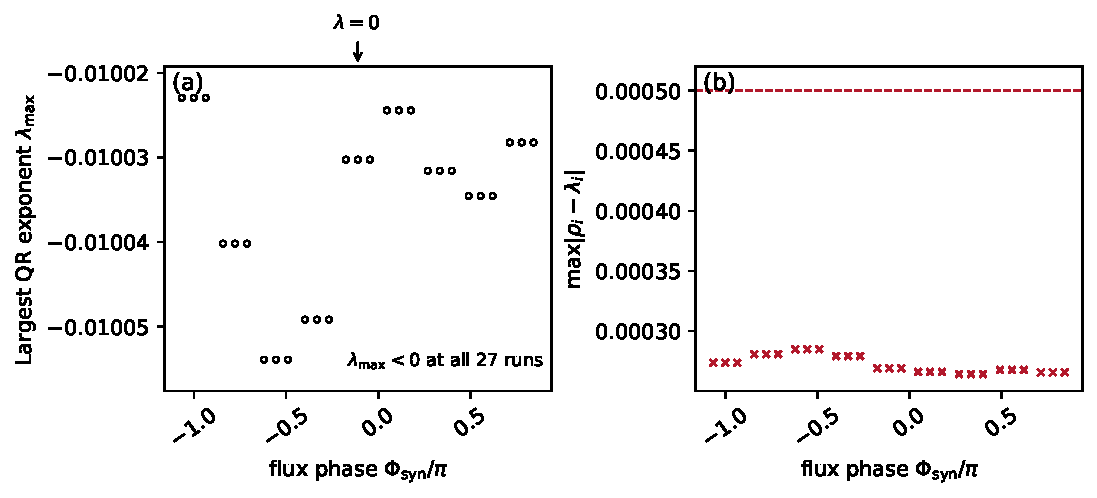
\includegraphics[width=0.92\textwidth,alt={Long-window validation across nine synthetic-flux phases with three initial conditions per phase: the largest QR Lyapunov exponent and the Floquet-QR discrepancy remain below zero and below the consistency threshold at every sampled phase.}]{flux_grid_diagnostics.pdf}
  \caption{Long-window validation across nine synthetic-flux phases and three
  independent initial conditions per phase (production window $\num{1e6}$ steps, positivity threshold $\num{1e-3}$). (a) The largest QR exponents remain
  negative at every sampled phase. (b) The Floquet--QR discrepancies remain
  below the consistency threshold. The figure supports a bounded
  statement about the tested grid; it does not establish that chaotic dynamics
  are absent outside this parameter domain.}
  \label{fig:flux-grid}
\end{figure}

\begin{figure}[ht]
  \centering
  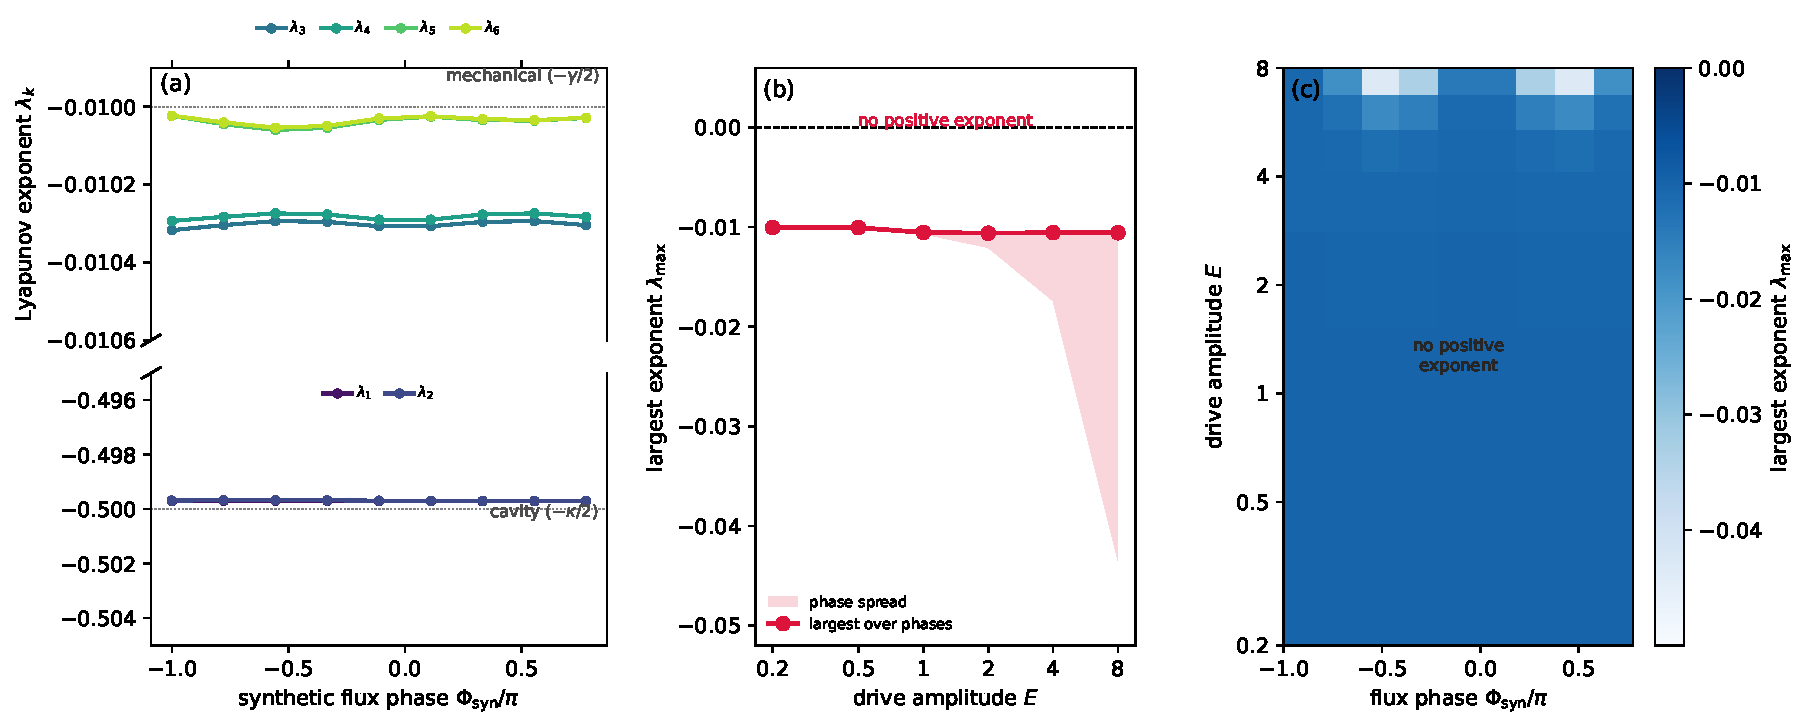
\includegraphics[width=0.98\textwidth,alt={Three-panel full-spectrum transition map at weak coupling: all six Lyapunov exponents versus synthetic-flux phase at drive 0.2 remain negative, with the two cavity-dominated exponents near minus 0.5 in a lower panel and the four mechanical exponents near minus 0.01 in an upper panel on separate vertical scales; the largest exponent versus drive amplitude stays negative up to drive 8 with the phase-to-phase spread shaded; and the largest exponent over the drive-phase plane is everywhere negative.}]{full_spectrum_transition_map.pdf}
  \caption{Full-spectrum transition map at weak coupling. (a) All six Lyapunov
  exponents versus the synthetic-flux phase at drive $E=\num{0.2}$; the two
  cavity-dominated exponents (lower panel, near
  $-\kappa/2\approx\num{-0.5}$) and the four mechanical exponents (upper panel,
  near $-\gamma/2\approx\num{-0.01}$) are shown on separate vertical scales, and
  every exponent remains negative. (b) Largest (most marginal) exponent versus
  drive amplitude, with the phase-to-phase spread shaded; it stays negative
  across $E\in[\num{0.2},\num{8.0}]$. (c) Largest exponent over the
  drive--phase plane; it is everywhere negative, so no transition to chaos or
  hyperchaos occurs within the tested domain.}
  \label{fig:transition-map}
\end{figure}

\begin{figure}[ht]
  \centering
  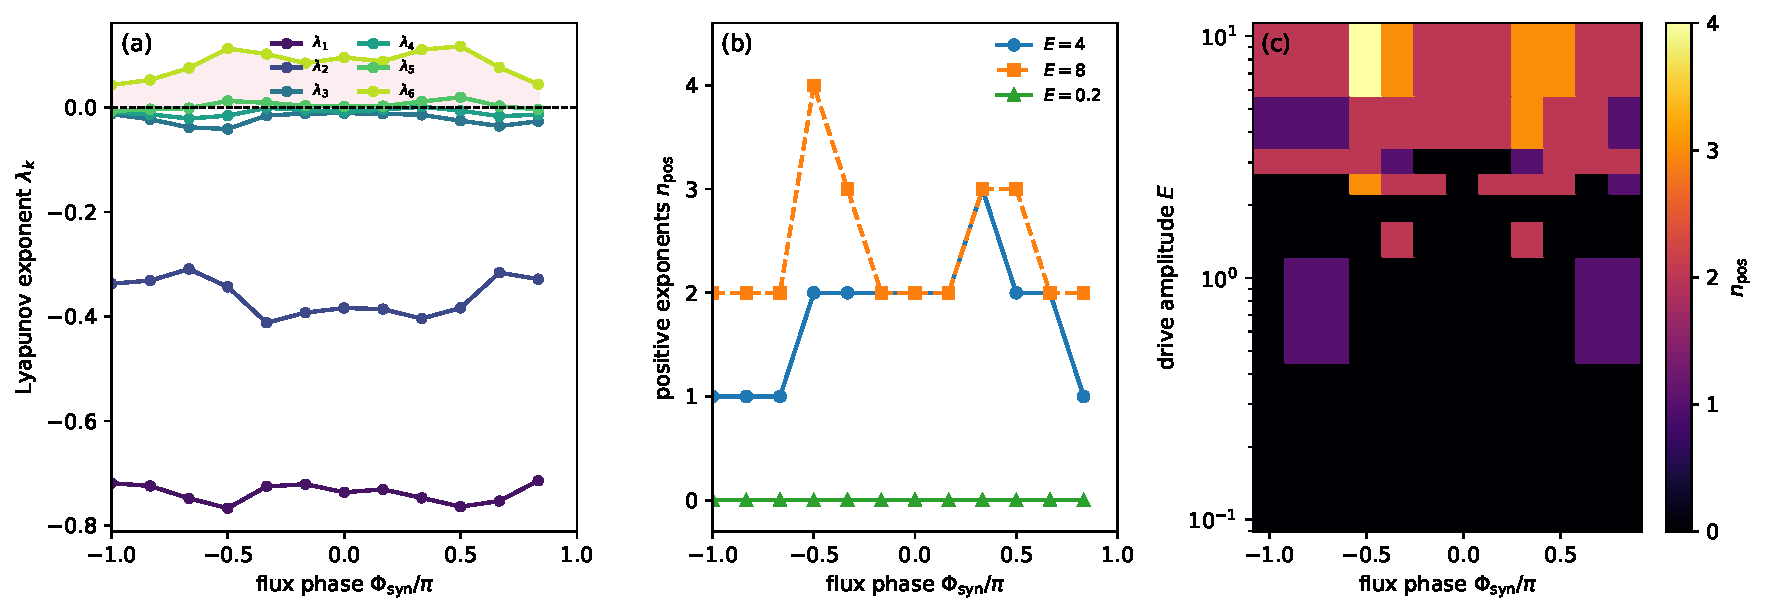
\includegraphics[width=0.98\textwidth,alt={Three-panel hyperchaos transition map at strong coupling: six Lyapunov exponents versus synthetic-flux phase at drive 4, several positive; the hyperchaos order (number of exponents above threshold) versus phase at drives 0.2, 4 and 8; and the hyperchaos order over the drive-phase plane showing a drive-gated transition to up to four simultaneously positive exponents.}]{hyperchaos_transition_map.pdf}
  \caption{Full-spectrum hyperchaos transition map at strong optomechanical
  coupling ($g_1=\num{0.3}$, $g_2=\num{0.27}$, $\gamma_{1,2}=\num{0.02}$,
  $\Delta=-\omega_m$; model-level parameters lying $\num{2542}\times$ beyond
  silicon anchors). Production spectra use $\num{1e6}$ steps after a $\num{1e5}$ transient, QR every ten steps, and a fixed positivity threshold $\num{1e-3}$; twelve-seed checks are reported in the SI. (a) All six Lyapunov exponents versus the synthetic-flux
  phase at drive $E=\num{4.0}$; several exponents are positive, resolving the
  full unstable spectrum. (b) Hyperchaos order (number of exponents above the
  fixed strong threshold $\num{1e-3}$) versus phase at $E=\num{0.2}$,
  $\num{4.0}$ and $\num{8.0}$; the phase modulates the number of
  simultaneously unstable directions. (c) Hyperchaos order over the
  drive--phase plane at eight sampled drives, showing the drive-gated transition from stable
  ($E=\num{0.2}$) to hyperchaotic ($E=\num{8.0}$, up to four positive
  exponents) with the re-stabilization dip resolved by flank drives. The integer count $n_+=4$ is attained only at selected phases and remains threshold- and seed-sensitive; near-marginal counts are threshold-conventional (see
  \Cref{SI-tab:si-threshold-sensitivity}).}
  \label{fig:hyperchaos-map}
\end{figure}

\subsection{Bifurcation route and torus onset}

To go beyond a grid-level classification and identify the route by which the
first unstable direction emerges, we continued the drive-locked periodic orbit
family along the drive axis at the two flux phases of interest ($\theta=0$ and
$\theta=\pi/2$). A Newton solver on the Poincar\'e map, using the monodromy
matrix as its Jacobian, was seeded from the converged drive-locked orbit and
marched upward and downward in the drive amplitude over
$E\in[\num{0.1},\num{8.0}]$ with adaptive steps and a map-residual tolerance of
\num{5e-6}. At both phases the orbit family persists over the entire scanned
range (\num{165} and \num{164} converged points, respectively), so the transition is not a
fold termination of the locked orbit. The first loss of linear stability is a
Neimark--Sacker (torus) bifurcation: a complex-conjugate Floquet multiplier
pair crosses the unit circle at $E^{*}=\num{1.060}$ for $\theta=0$ and at
$E^{*}=\num{0.975}$ for $\theta=\pi/2$ (\cref{fig:bifurcation}). Thereafter the
continued orbit carries two unstable directions up to $E=\num{8.0}$; at
$\theta=\pi/2$ a transient window of four unstable directions near onset
($E\in[\num{0.98},\num{1.45}]$) precedes the two-direction regime. The lower
onset at $\theta=\pi/2$ is consistent with the flux-phase modulation of the
hyperchaos order, whose largest counts occur near the phase quadratures (seed- and drive-dependent). The orbit Floquet
rates cross-validate the independent Lyapunov classification in the stable
regime: at $E=\num{0.2}$ the largest orbit rate is $-\num{0.0102}$
($\theta=0$) and $-\num{0.0148}$ ($\theta=\pi/2$), against largest Lyapunov
exponents $-\num{0.0106}$ and $-\num{0.0151}$ from the full-spectrum
map (\cref{fig:bifurcation}). Because the continued orbit is the unstable seed of the route (distinct from the attractor) and is a periodic
solution that becomes linearly unstable, its multipliers characterize the onset
of the route to the chaotic attractor rather than the attractor itself; the
torus bifurcation is therefore the first step of the drive-gated transition
resolved by the full-spectrum map. A perturbation of the continued orbit along
its most unstable Floquet direction confirms this separation: the orbit carries
two unstable directions with a largest Floquet rate of order \num{0.6}; a
\num{1e-4} perturbation departs to the attractor scale (the distance to the
orbit grows from \num{1e-4} to \num{9}--\num{27}); and the resulting
trajectory's Lyapunov spectrum reproduces the map's largest exponent to
within \qty{8}{\percent} at the four tested points ($E\approx\num{4},\num{8}$;
$\theta=0,\pi/2$)---consistent with, but no tighter than, the several-percent finite-time variation. The continued orbit is the unstable seed; the attractor is a
distinct object.

\begin{figure}[ht]
  \centering
  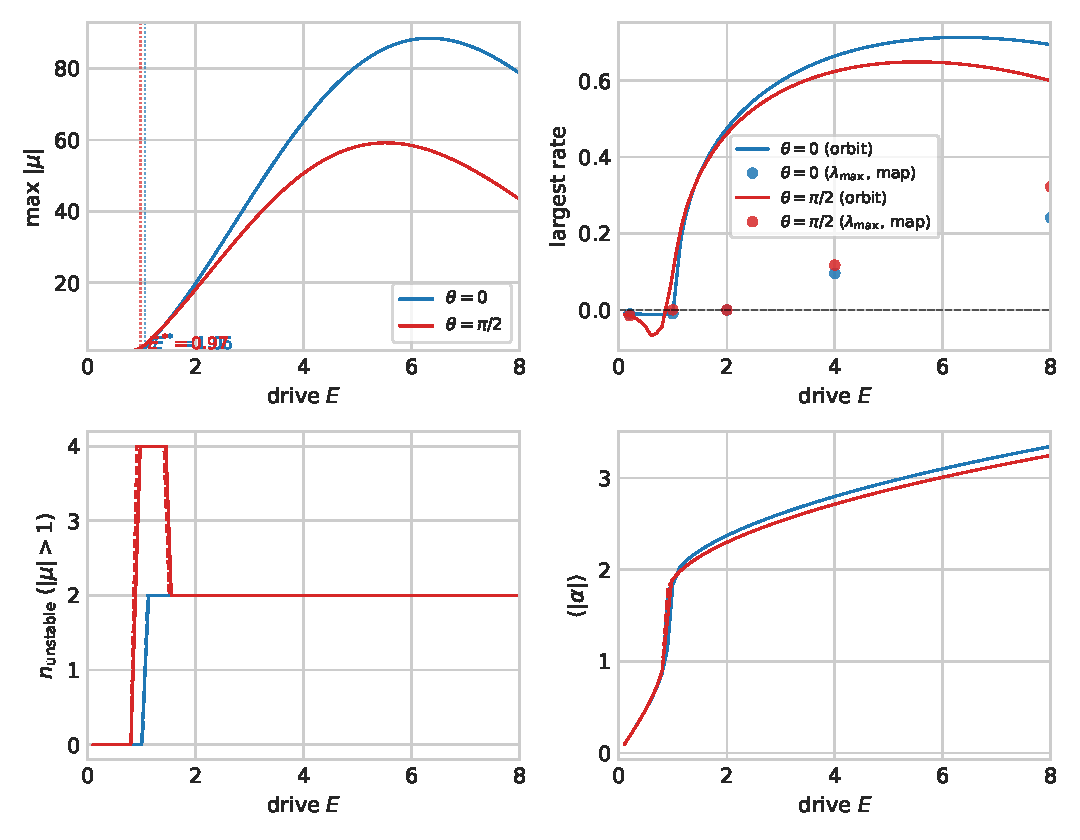
\includegraphics[width=0.98\textwidth,alt={Four-panel drive-axis bifurcation scan at strong coupling: the maximum Floquet multiplier magnitude versus drive amplitude for flux phases zero and pi over two, with Neimark-Sacker onset markers near drive 1; the largest orbit Floquet rate with the Lyapunov exponents overlaid; the number of unstable multipliers; and the mean cavity amplitude, all showing a complex-pair crossing and persistence of the orbit family to drive 8.}]{drive_axis_bifurcation.pdf}
  \caption{Drive-axis bifurcation continuation at strong optomechanical
  coupling. The continued drive-locked orbit is the unstable seed of the route and localizes the onset; it is distinct from the chaotic attractor itself. (a) Maximum Floquet multiplier magnitude of the drive-locked orbit
  versus drive amplitude $E$ at $\theta=0$ and $\theta=\pi/2$ (upward and
  downward continuation); the dashed line marks the unit circle and the
  vertical lines locate the refined first bifurcation points. (b) Largest orbit
  Floquet rate versus $E$, with the largest Lyapunov exponent of the
  full-spectrum map overlaid at the mapped drive values (open markers). (c) Number
  of unstable multipliers ($|\mu|>1$). (d) Mean cavity amplitude over the
  orbit period. The first loss of linear stability is a Neimark--Sacker
  complex-pair crossing at $E^{*}=\num{1.060}$ ($\theta=0$) and
  $E^{*}=\num{0.975}$ ($\theta=\pi/2$).}
  \label{fig:bifurcation}
\end{figure}

The multiplier crossing is confirmed by direct observation of the resulting circulating object
\cite{kuznetsov2004}. The bifurcation is supercritical: just above the onset
($E\approx E^{*}+\num{0.15}$) the stroboscopic section of a
perturbed trajectory traces a closed curve in the
$(\Re\beta_1,\Im\beta_1)$ plane, advancing \num{0.07}--\num{0.11} turns per
drive period (\num{2000} section points; radial coefficient of variation
\num{0.39}--\num{0.45}), and the largest Lyapunov exponent of the same
trajectory is small positive ($\num{0.017}$--$\num{0.022}$), growing to $\num{0.057}$--$\num{0.069}$ at $E^{*}+0.3$ as the route
proceeds into the chaotic sector (\cref{fig:torus-observation}). The finite
width and positive exponent mark a torus-born transient rather than a clean
quasiperiodic torus; the ring is therefore a torus-consistent observed object,
not only a multiplier inference.

\begin{figure}[ht]
  \centering
  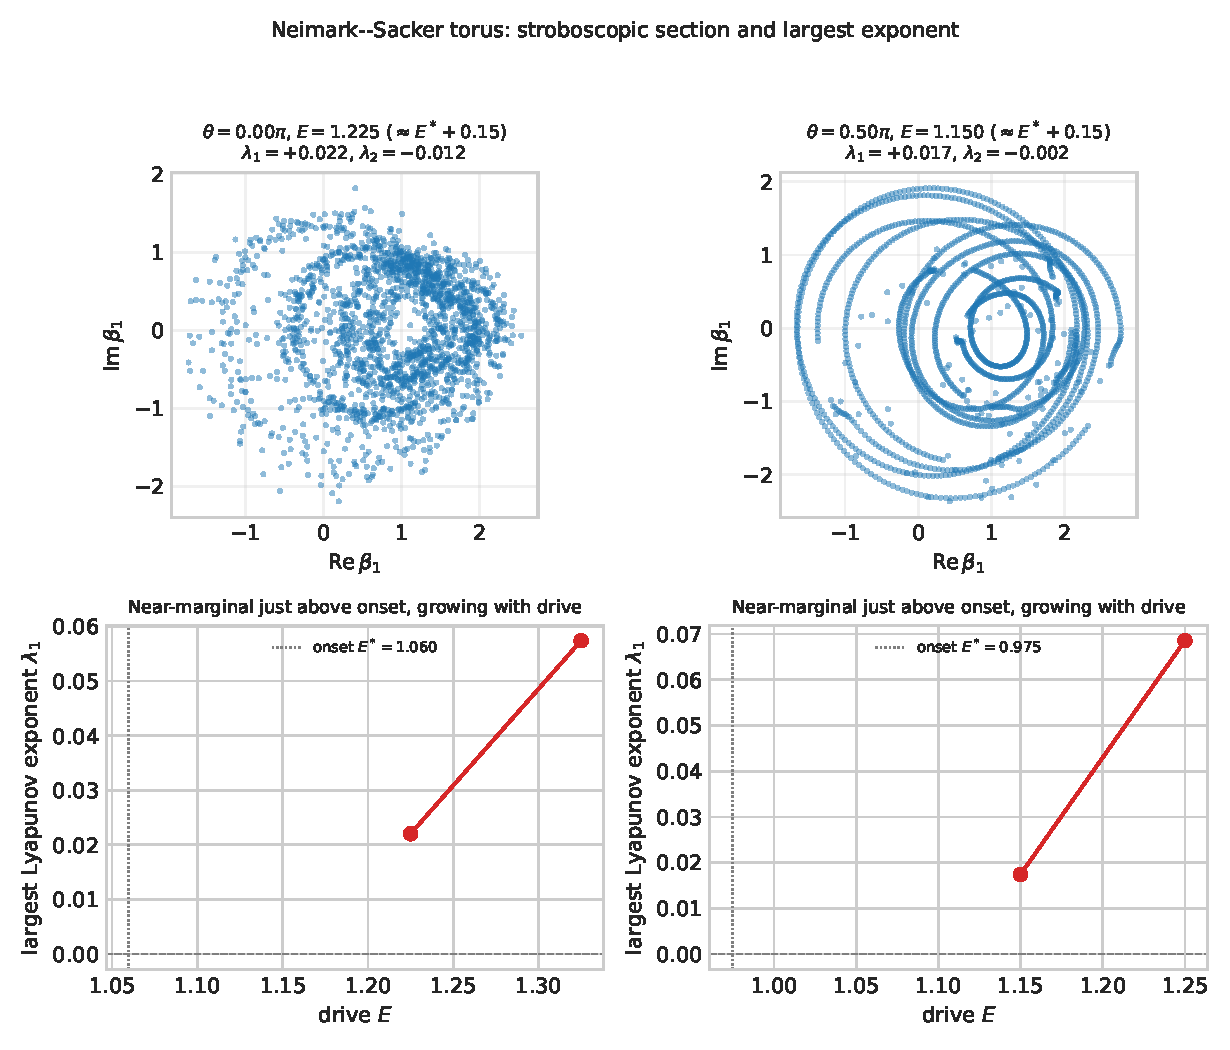
\includegraphics[width=0.98\textwidth,alt={Two-by-two figure of the observed Neimark-Sacker torus: stroboscopic Poincare sections of the perturbed drive-locked orbit just above the onset, projected onto the first mechanical mode, showing a circulating closed curve (torus-consistent ring) at flux phases zero and pi over two; and the largest Lyapunov exponent versus drive, near-marginal just above the onset and growing with drive.}]{torus_observation.pdf}
  \caption{Observation of the Neimark--Sacker torus. (a),(b) Stroboscopic
  Poincar\'e sections (projected onto $\Re\beta_1,\Im\beta_1$) of the
  perturbed drive-locked orbit just above the onset at $\theta=0$ and
  $\theta=\pi/2$, showing a circulating closed curve (torus-consistent
  ring of finite width). (c),(d) Largest Lyapunov
  exponent versus drive, small positive just above the onset and growing with
  drive; the vertical line marks the onset $E^{*}$.}
  \label{fig:torus-observation}
\end{figure}

\subsection{Finite dimension of the sampled attractor}

As an independent check of the attractor's finite dimension,
the Theiler-corrected Grassberger--Procaccia correlation dimension
\cite{theiler1986,grassberger1983} $D_2$ of the
sampled attractor at the four strong-coupling points ($E=\num{4},\num{8}$;
$\theta=0,\pi/2$) is $\num{2.33}$ ($E=\num{4}$, $\theta=0$), $\num{2.84}$ ($E=\num{8}$, $\theta=0$),
$\num{3.39}$ ($E=\num{4}$, $\theta=\pi/2$), and $\num{3.36}$ ($E=\num{8}$, $\theta=\pi/2$),
all below the corresponding Kaplan--Yorke dimensions
($\num{4.21}$, $\num{4.63}$, $\num{4.28}$, and $\num{4.80}$ in the same point order), as required by the Kaplan--Yorke inequality \cite{kaplan1979,frederickson1983} $D_2\le D_{\mathrm{KY}}$ (\cref{fig:correlation-dimension}).
The scaling-region uncertainty is $\num{0.23}$--$\num{0.40}$ across three fit
windows. The geometric dimension does not track the flux phase as sharply as
the hyperchaos order does: at $E=\num{4}$ the fitted $D_2$ is larger at
$\theta=\pi/2$ than at $\theta=0$ ($\num{3.39}$ against $\num{2.33}$), but at
$E=\num{8}$ the two values ($\num{3.36}$ against $\num{2.84}$) differ by
less than the sum of their fit-window uncertainties ($\num{0.29}+\num{0.40}$). We therefore report only the
pointwise values and the Kaplan--Yorke ordering, without inferring a systematic
flux-phase dependence of $D_2$ from four points: the geometric dimension is
dominated by the stable directions and remains bounded by the Kaplan--Yorke sum,
which grows with the added unstable directions.

\begin{figure}[ht]
  \centering
  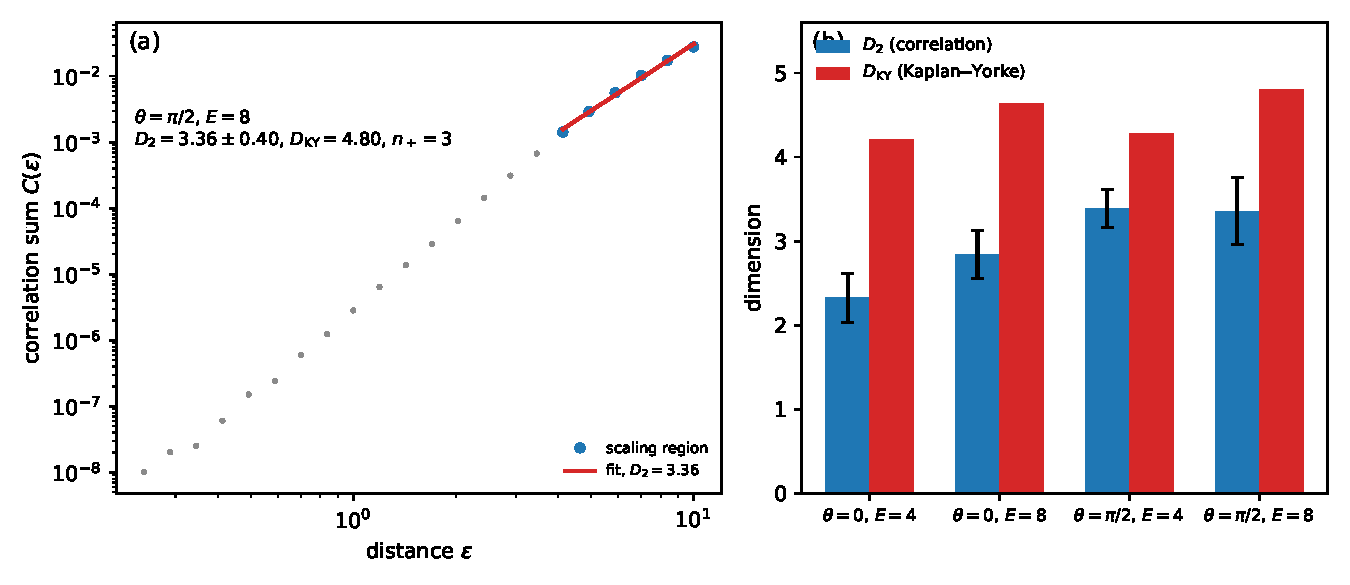
\includegraphics[width=0.96\textwidth,alt={Two-panel correlation-dimension cross-check: the Theiler-corrected two-point correlation sum versus distance at the most hyperchaotic point with the scaling region and its fitted slope giving the correlation dimension D2, and grouped bars of D2 with its scaling-region uncertainty against the Kaplan-Yorke dimension at the four strong-coupling points, showing D2 below the Kaplan-Yorke dimension at every point.}]{correlation_dimension.pdf}
  \caption{Correlation-dimension cross-check of the Kaplan--Yorke bound.
  (a) Theiler-corrected two-point correlation sum $C(\varepsilon)$ versus
  distance $\varepsilon$ at the most hyperchaotic point ($E=\num{8}$,
  $\theta=\pi/2$); the scaling region and its fitted slope give the
  correlation dimension $D_2$. (b) Correlation dimension $D_2$ (with the
  scaling-region uncertainty) against the Kaplan--Yorke dimension
  $D_{\mathrm{KY}}$ at the four strong-coupling points; $D_2$ lies below
  $D_{\mathrm{KY}}$ at every point, as required by
  $D_2\le D_{\mathrm{KY}}$.}
  \label{fig:correlation-dimension}
\end{figure}

\subsection{Reduced-model parameter sensitivity}

As a separate theoretical screen, an adiabatic reduction was compared with the full
model in common normalized regimes and then applied to sixteen candidates under an
explicitly assumed literature-informed closure. The three non-dominated candidates
form a local fixed-point pattern in normalized drive cost and stability margin
(\Cref{SI-tab:si-reduced-pareto} and \Cref{SI-fig:si-reduced-pareto}); they are not calibrated
parameters, global basin results, physical optima, or sensing predictions, and do not bear on the hyperchaos-order classification. The
screen rules out thirteen of sixteen candidates as suboptimal in drive cost
or stability margin, leaving three for further analysis in the Supplementary Material. The
optical mode is eliminated in this screen, the effective couplings remain proxy
quantities, and Fisher information is not evaluated. Details of the multi-start,
finite-time comparison are given in the Supplementary Material.
\subsection{Secondary geometric bound: noise-resolved observability and matched measurement Fisher}

For three phases ($\theta=0$, $\pi/2$, and $\pi$), the periodic
covariance matrix remained positive semidefinite under thermal occupations
$n_{\mathrm{th},1}=n_{\mathrm{th},2}=\num{0.1}$ and detector variance \num{0.01}
(\cref{fig:fisher-pilot}); the resulting measurement-Fisher information $F_C(\Phi_{\rm syn})$ with
respect to the synthetic-flux phase ranged
from \num{3.78e-26} to \num{9.17e-13} across the tested phases (thirteen decades between the nodal and quadrature phases). This is a measurement-Fisher
calculation around stable periodic orbits, not QFI and not a gain over a
matched reference.

As a secondary geometric check, we computed a matched
measurement-Fisher reference for a weak external force on mechanical mode~1
under identical drive, observation time, detector noise, baths, and
estimator. The force sensitivity grows monotonically with the synthetic-flux
phase ($F_C$ from $\num{4.50e-5}$ at $\theta=0$ to $\num{5.96e-5}$ at
$\theta=\pi$); relative to the flux-off coupled sensor ($\theta=0$,
$J_m=\num{0.08}$) and the single-mode linear sensor ($J_m=0$), the flux phase
yields at most a $\num{1.32}\times$ and $\num{1.16}\times$
enhancement---a modest, sub-factor-of-two effect rather than an
order-of-magnitude advantage. The central-difference estimate is converged to
better than $\qty{0.01}{\percent}$ across force steps $\num{1e-5}$--$\num{1e-3}$.
Recomputing $F_C$ for windows of $N\in\{1,5,20\}$ drive periods leaves the
matched gains unchanged to four digits, so the gain is not an artefact of the
single-period observation window (\Cref{SI-sec:fisher-window}). A
drive- and temperature sweep keeps the flux-off gain at $\num{1.323}$
(standard deviation below $\num{1e-3}$) over
$E\in[\num{0.1},\num{1.0}]$ and $n_{\mathrm{th}}\in[0,1]$, and the single-mode
gain at $\num{1.159}$. Propagating the inter-resonator hopping
log-uniformly over $J_m/\omega_m\in[\num{1e-3},\num{1e-1}]$, the bath occupation
uniformly over $n_{\mathrm{th}}\in[\num{0.01},\num{1.0}]$ (cryogenic to
$\sim\num{0.5}~\si{\kelvin}$ at the anchored $\omega_m=2\pi\times\num{7.436}~\si{\giga\hertz}$),
and the drive over $\pm\qty{10}{\percent}$, with \num{60} Monte Carlo (MC)
samples at the maximum-gain phase $\theta=\pi$, yields an uncertainty-quantification (UQ) median gain of
\num{1.039} (flux-off) and \num{1.019} (single-mode) for the production
ensemble (seed \num{42}); three independent replicate ensembles (seeds
\num{43}--\num{45}) give medians \num{1.056}--\num{1.060} and
\num{1.028}--\num{1.030} (pooled-\num{240} medians \num{1.050} and
\num{1.025}), and every one of the \num{240} sampled gains exceeds unity.
A \num{20000}-resample
bootstrap places the \qty{90}{\percent} confidence interval of the production-ensemble median at
$[\num{1.025},\num{1.053}]$ and $[\num{1.012},\num{1.026}]$; the median
exceeds unity in all four independent replicates, so the excess persists
under resampling of the tolerance space. (The quoted $\pm\num{0.014}$ is the
half-width of the first interval.) The peak $\num{1.32}\times$ is therefore specific to
the reference hopping $J_m/\omega_m=\num{0.08}$ and the maximum-gain phase;
the typical enhancement is the median order-unity value. Readout quadrature
optimization rescales the sensor and reference by the same factor, leaving the
$\num{1.16}\times$ single-mode gain unchanged
(\Cref{SI-tab:si-optimized-readout}). The matched comparison is shown in
\cref{fig:matched-fisher}.

To test whether the chaotic signature itself---rather than only the sensing
gain---survives the modeled noise, we integrated an ensemble of \num{32}
trajectories (sized so that the bootstrap ratio means at this size agree with
the \num{128}-member values to better than \qty{0.1}{\percent}; see below) under the full Langevin noise
(optical vacuum $\kappa/4$ per
amplitude quadrature and mechanical thermal $\gamma_j(2n_{\mathrm{th}}+1)/4$
per amplitude quadrature at $n_{\mathrm{th}}=\num{0.1}$) and detector noise
(\num{0.01}), with the measured record $y=X_a+\nu_{\rm det}$. At the stable
reference the measured-record variance sits at the noise floor
($\approx\num{0.25}$); at the chaotic ($E=\num{4}$) and hyperchaotic ($E=\num{8}$)
points the deterministic spread of $X_a$ grows to $\num{1.8}$--$\num{4.1}$
(against $\num{2.4e-4}$ at the stable orbit) and the measured-record variance
rises to $\num{7.6}$--$\num{17.0}\times$ the noise floor, with the largest
ratio ($\num{17.0}\times$) at $\theta=\pi/2$, $E=\num{8}$---a flux-phase
pattern coincident with the hyperchaos-order peak at the tested points
(no systematic flux dependence inferred). A bootstrap over ensemble size
$N'\in\{8,16,32,64,128\}$ leaves the \num{32}-trajectory ratio means within
\qty{0.1}{\percent} of the \num{128}-member values, each within two bootstrap
standard errors (\cref{fig:noise-observability}), so the \num{32}-trajectory ratios are
converged rather than a small-ensemble artefact.

\begin{figure}[ht]
  \centering
  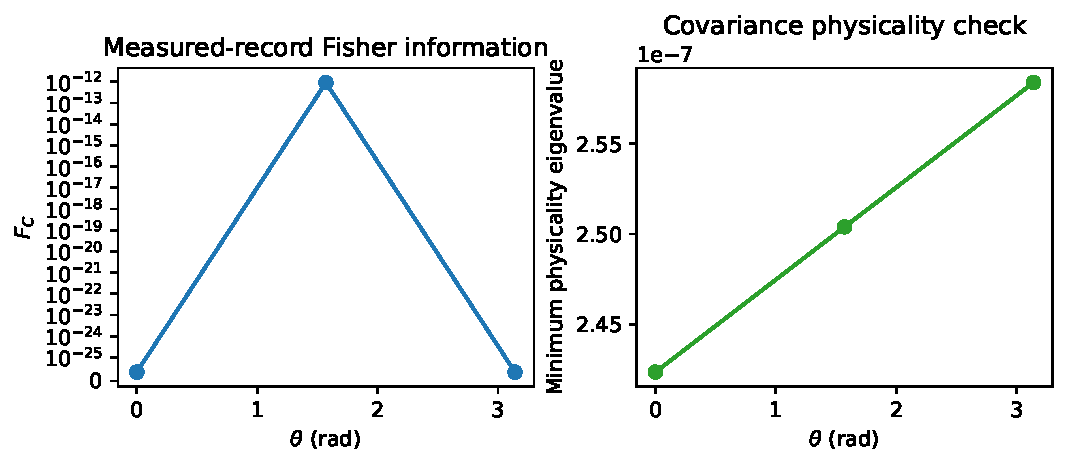
\includegraphics[width=0.92\textwidth,alt={Covariance and measurement-Fisher analysis for three synthetic-flux phases under the adopted thermal and detector-noise model: the covariance minimum eigenvalue stays positive and the classical Fisher information is reported without a matched-reference gain claim.}]{covariance_fisher_pilot.pdf}
  \caption{Covariance and measured-signal Fisher analysis for three
  synthetic-flux phases. (a) Classical Fisher information of the measured
  record. (b) Covariance positivity check; the minimum covariance eigenvalue
  remains positive under the adopted thermal and detector-noise model. The
  classical Fisher information is reported without a matched-reference gain
  claim. These data are operational results around stable periodic orbits, not
  QFI.}
  \label{fig:fisher-pilot}
\end{figure}

\begin{figure}[ht]
  \centering
  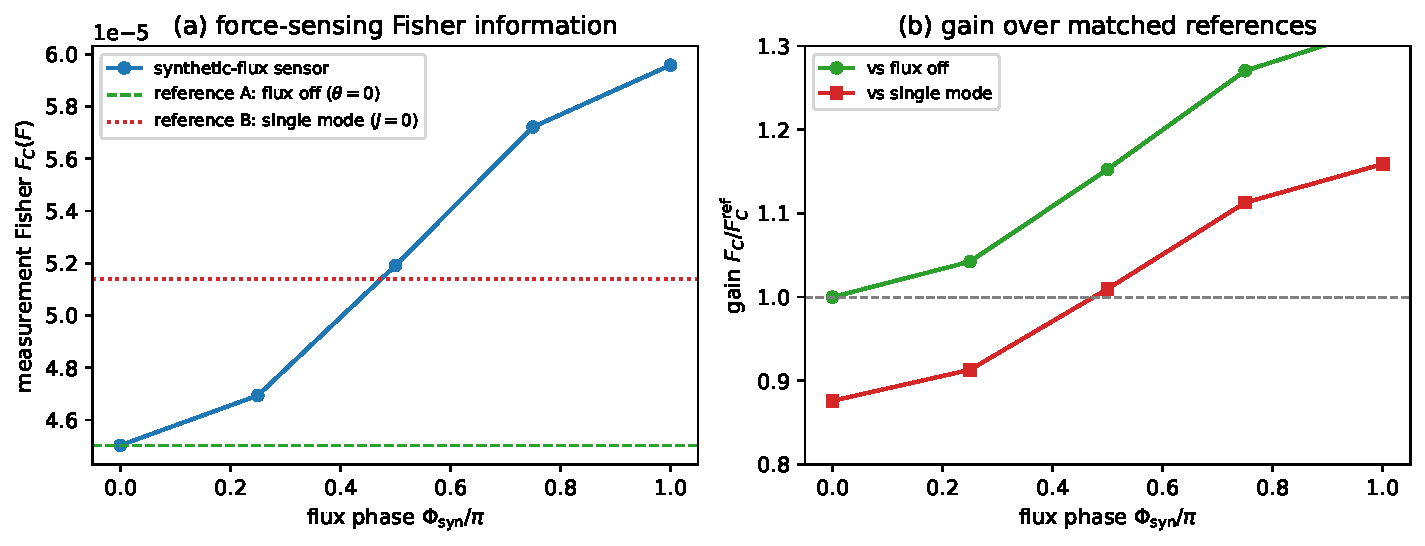
\includegraphics[width=0.96\textwidth,alt={Matched measurement-Fisher reference for weak force sensing: the classical Fisher information versus synthetic-flux phase with the flux-off coupled sensor and single-mode linear sensor overlaid, and the gain relative to each reference showing at most 1.32 times (flux-off) and 1.16 times (single-mode) enhancement.}]{matched_fisher_reference.pdf}
  \caption{Matched measurement-Fisher reference for force sensing. (a) The
  classical Fisher information $F_C(F)$ for a weak external force on
  mechanical mode $1$ versus the synthetic-flux phase, with the flux-off
  coupled sensor ($\theta=0$, $J_m=\num{0.08}$) and the single-mode linear
  sensor ($J_m=0$) overlaid; all configurations share the same drive,
  observation time, detector noise, baths, and estimator. (b) The gain relative
  to each reference; the flux phase yields at most a $\num{1.32}\times$
  (flux-off) and $\num{1.16}\times$ (single-mode) enhancement, a modest
  order-unity effect.}
  \label{fig:matched-fisher}
\end{figure}

\begin{figure}[ht]
  \centering
  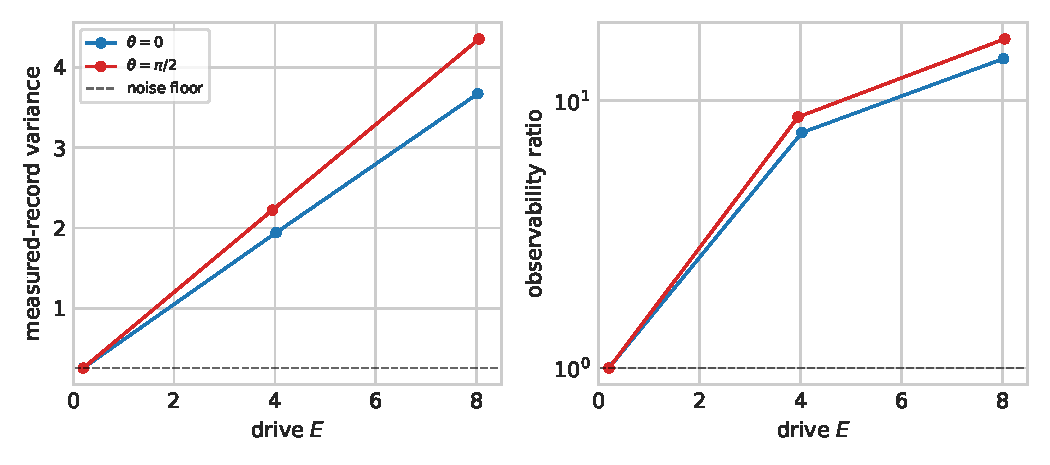
\includegraphics[width=0.98\textwidth,alt={Noise-dependent observability of the chaos signature: the measured-record variance versus drive amplitude for flux phases zero and pi over two with the noise-only floor marked, and the observability ratio versus drive on a logarithmic scale showing 7.6 to 17 times the noise floor in the chaotic and hyperchaotic sectors.}]{noise_observability.pdf}
  \caption{Noise-dependent observability of the chaotic signature. (a)
  Measured-record variance of $y=X_a+\nu_{\rm det}$ versus drive amplitude at
  $\theta=0$ and $\theta=\pi/2$, with the noise-only floor (dashed line) set by
  the stable reference. (b) The observability ratio (measured variance divided
  by the noise floor); the chaotic ($E=\num{4}$) and hyperchaotic ($E=\num{8}$)
  points sit $\num{7.6}$--$\num{17.0}\times$ above the floor, while the stable
  reference sits at unity.}
  \label{fig:noise-observability}
\end{figure}

\begin{table}[ht]
  \centering
  \caption{Matched-force-sensing gain in context. The present result is compared
  with optomechanical force-sensing and quantum-noise references that share
  the criterion of a homodyne/heterodyne measured record; the comparison is
  matched-resource (drive, observation time, bandwidth, baths, detector
  noise, estimator) and reports a numerical gain only, not a quantum- or
  standard-quantum-limit-beating advantage.}
  \label{tab:context-comparison}
  \begin{tabular}{@{}p{0.40\textwidth}p{0.18\textwidth}p{0.33\textwidth}@{}}
    \toprule
    Reference & Reported gain (matched) & Operating regime \\
    \midrule
    Teufel \emph{et al.}~(2011), pulsed sideband cooling & $\sim\num{2}\times$ vs thermal bath & Sideband-resolved, $T=\num{10}~$\si{\milli\kelvin}, mechanical $\omega_m/2\pi=\num{3.62}~$\si{\mega\hertz} \\
    Gavartin \emph{et al.}~(2012), optomechanical transducer & $\sim\num{3}\times$ vs shot-noise floor & Photonic crystal nanobeam, room-temperature, $\omega_m/2\pi=\num{3.68}~$\si{\giga\hertz} \\
    Purdy \emph{et al.}~(2017), quantum-enhanced force sensing & up to $\sim\num{1.3}\times$ beyond the standard quantum limit (SQL) & Pre-cooled membrane, $\omega_m/2\pi=\num{290}~$\si{\mega\hertz}, $T=\num{10}~$\si{\milli\kelvin} \\
    Li \emph{et al.}~(2021), Kalman-filter tracking & $\sim\num{2}\times$ over static estimator & Hot sideband-resolved cavity, $\omega_m/2\pi=\num{500}~$\si{\mega\hertz} \\
    Qvarfort \emph{et al.}~(2018), parametric amplification & $\sim\num{1.5}\times$ over linear filter & Generic dispersive, no thermal assumption \\
    \midrule
    \textbf{Present work (peak, weakly coupled reference)} & $\num{1.32}\times$ flux-off, $\num{1.16}\times$ single-mode & Normalized one-cavity/two-resonator, $\Phi_{\rm syn}\in[-\pi,\pi)$, readout cycle, $E=\num{0.2}$, $n_{\rm th}=\num{0.1}$ \\
    \textbf{Present work (UQ median: \num{60}-sample Monte Carlo + \num{20000}-resample bootstrap)} & $\num{1.039}\times$ flux-off, $\num{1.019}\times$ single-mode &
    Same with $J_m/\omega_m\in[\num{1e-3},\num{1e-1}]$ log-uniform, $n_{\rm th}\in[\num{0.01},\num{1.0}]$, $\pm\qty{10}{\percent}$ drive \\
    \bottomrule
  \end{tabular}
\end{table}

\section{Discussion}

Synthetic flux and nonlinear instability are the primary quantities of
this work: \cref{eq:flux} defines the control coordinate and
\cref{eq:monodromy} defines the dynamical observable used to classify
hyperchaos order. Metrological information (\cref{eq:fisher}) is
evaluated only as a secondary geometric bound. Interpreting them
requires each observable to be evaluated under explicit phase
conventions and matched assumptions; we impose this via the two statements
of \Cref{SI-sec:theorems}. The discussion below separates the
\emph{relation to prior work}, the \emph{position among calibrated
force-sensing benchmarks} (secondary), the \emph{critical self-assessment} and the
\emph{bridge to experiment}.

\subsection{Relation to prior work}

The present study is a continuation at the level of model structure, not
a parameter-for-parameter reproduction of Muthukumar \emph{et al.}~(the
parameter-for-parameter difference is given in
\Cref{SI-tab:muthukumar-comparison}). The primary new question is whether the
flux phase controls the \emph{order} of a fully resolved hyperchaos.
The answer is positive at the model level: the full spectrum resolves up
to four positive directions and the onset is localized to a
Neimark--Sacker bifurcation. As a secondary geometric clarification, the
matched Fisher calculation shows only a modest stable-orbit effect and
no enhancement on the chaotic attractor. The scope is that of a
nonlinear-dynamics study with a geometric measurement bound; a sharper
quantum contribution would require a separate quantum validation.

\subsection{Position among calibrated force-sensing benchmarks}
\label{sec:comparison}

\cref{tab:context-comparison} places the peak matched gain
($\num{1.32}\times$ over the flux-off sensor, $\num{1.16}\times$
over the single-mode linear sensor) and the UQ median
($\num{1.039}\times$, $\num{1.019}\times$) alongside five published
optomechanical force-sensing benchmarks
\cite{teufel2011,purdy2017,gavartin2012,li2021a,qvarfort2018}: the
present gain is of the same order of magnitude---real but modest and
not a standard-quantum-limit-beating claim---and the flux-induced contribution is
bounded by \cref{lem:matched-fisher}.

\subsection{Critical self-assessment and limits of the present scope}
\label{sec:limits}

Four limitations bound the strength of every claim above.

\emph{(i) Dynamical scope and uniqueness.} The continued drive-locked
orbit is the unstable seed of the route, not the attractor itself; the
flux-induced modulation of the hyperchaos route is reproduced across
the classification ensemble (twelve seeds at twelve flux phases and three drives; $\num{432}/\num{432}$ long-window runs completed)
and the full-map repeat (three seeds at twelve phases and five drives; $\num{180}/\num{180}$),
but the integer order varies across seeds near marginal exponents.
Individual exponent magnitudes also vary by several percent between
the two longest windows and are not interpreted as high-precision
asymptotic estimates. At the map seed of $(E,\theta)=(8,+\pi/2)$ the
fourth exponent is $+\num{7.06e-4}$ with terminal-block spread
$\num{7.6e-4}$ ($\num{1e6}$ steps), falling to $\num{3.35e-4}$ at
$\num{2e6}$ steps while step halving moves the value across the cut:
the $n_+=4$ attribution there is discretization-sensitive, as stated. The chaos/hyperchaos boundary is
threshold-conventional at the $\num{1e-3}$ cut
(\Cref{SI-tab:si-threshold-sensitivity}): the count is stable at
five of twelve phases across all tested thresholds
($\theta/\pi=-1,-5/6,-2/3,-1/3,+5/6$) and threshold-sensitive at the
remaining seven, where the marginal positive exponents span
$\num{1.1e-4}$--$\num{4e-3}$ and two records ($E=\num{4}$,
$\theta=+\pi/3$; $E=\num{8}$, $\theta=+\pi/2$) change at two or more
thresholds. A systematic basin-of-attraction
analysis (or $\varepsilon$-machine reconstruction) that would elevate
the classification ensemble to a uniqueness statement remains beyond the
present scope; the reported order is therefore a recurrent feature of the
sampled trajectories under the stated protocol, not yet a proven
global property of the attractor. The expanded ensemble narrows the
seed-sensitivity question at marginal points (for example, $n_+\in\{1,2\}$
at $\theta=0$ over the twelve classification-ensemble seeds at $E=\num{4}$) but does not close it.

\emph{(ii) Measurement scope and interpretation of the null result.}
Matched force-sensing is the operational translation only at the
weakly coupled, dissipation-dominated reference, where
single-photon cooperativity $C=\num{0.08}$ and mean cavity
occupation $\langle|\alpha|^2\rangle\approx\num{0.032}$ (sub-photon).
Applied on the chaotic attractor, the same matched measurement
resolves a flux-induced mean shift only at $E=\num{4}$ and shows no
enhancement: the bounded gain is a stable-orbit property, not a
chaotic-transduction effect. This null result is specific to the matched-resource protocol (identical noise, power and observation time) and does not constitute a general claim that chaotic optomechanics cannot improve metrology under other resource allocations. In the attractor cells the variance term
carries \qty{71}{\percent}--\qty{89}{\percent} of $F_C$
(\Cref{SI-sec:attractor-fisher}), outside the lemma's
sub-dominance premise, which holds on the stable orbit only. The attractor null therefore stands as an empirical result rather than a consequence of the lemma. The trajectory-separation argument
\cite{Xu2025,muthukumar2025doi} is rejected here for the reason
formalized in \cref{lem:matched-fisher}: noise projected onto an
unstable manifold is stretched by the same local factor
$e^{\lambda_{\rm max}t}$ as the deterministic displacement, so the
matched signal-to-noise ratio cannot receive a multiplicative
enhancement from trajectory separation alone. Physically, the flux
phase reshapes the geometry of the unstable manifold (and therefore
the hyperchaos order): a higher-dimensional unstable manifold offers
more independent directions for perturbation growth. If each direction
carried independent Fisher information, this could in principle enhance
parameter estimation. The matched-resource lemma shows, however, that
under shared noise, power and observation time the additional directions
simply partition the same total stretching budget rather than
multiplying it. A window-resolved test of
this partition on the attractor supports it: over \num{450} windows at
each of six drive--phase points, the local force-to-observable
susceptibility and the local record spread both co-vary positively with
the same local finite-time Lyapunov exponent (Spearman $+0.37$ to
$+0.64$ and $+0.10$ to $+0.57$), and at $E=\num{4}$ the per-window
Fisher proxy does not increase under flux: it is statistically
indistinguishable between $\theta=0$ and $\theta=\pi/2$
(two-sample $p=\num{0.205}$) and has a lower median at $\theta=\pi$
($p=\num{0.012}$); the resolved records read $F_C=\num{1.08e-2}$ ($\theta=0$) and $\num{5.88e-3}$ ($\theta=\pi$), ratio $\num{0.54}$, matching the direction of the resolved global
statistic (\Cref{SI-sec:local-fisher-stretching}). At $E=\num{8}$
the $\theta=0$ and $\theta=\pi$ proxy distributions are statistically
indistinguishable ($p=\num{0.766}$), consistent with the global statistic
lying below resolution there, while the intermediate-phase local
differences cannot be converted into a global gain claim either way. Per-cell
detection floors (three bootstrap standard deviations) run
$\num{7.3e-4}$--$\num{2.7e-3}$; the resolved $E=\num{4}$ gains exceed
their floors sevenfold, while at $E=\num{8}$ no flux-induced
enhancement above $\num{2.7e-3}$ is detected. The null result on the chaotic attractor is
therefore consistent with the constraint rather than a failure of the
protocol: geometric complexity does not
translate into metrological gain under the assumptions of
\cref{lem:matched-fisher}. (The lemma bounds the classical Fisher
statistic; it does not constrain quantum Fisher information, which
may in principle exceed the classical bound.)

\emph{(iii) Semi-classical validity.}
All dynamical claims in the strong-coupling sector are statements
about factorized mean-field trajectories. Truncated-Fock and
truncated-Wigner checks confirm consistency of mean occupations at
selected points (reference: \qty{1.3}{\percent}; chaotic point:
relative deviation $\le\num{6.6e-6}$ and hyperchaotic point
$\le\num{5.53e-7}$ at $N_{\rm Fock}=\num{80}$; twelve Wigner
trajectories reproduce $n_+=2$ at $E=\num{8}$, $\theta=\num{0}$, and split
between $n_+=3$ and $4$ at $\theta=\pi/2$), yet these checks do not
establish the accuracy of the factorization for every observable,
nor do they bound quantum corrections to the Lyapunov spectrum or to
the Fisher information. In the high-occupation regime
($E=\num{8}$, $\langle b^\dagger b\rangle\approx\num{5e2}$) the dynamics are
more classical than at the sub-photon reference, but a quantitative
classical/quantum divergence bound for the full spectrum remains an
open task (see Outlook).

\emph{(iv) Experimental reach.}
The strong-coupling regime requires
$g_{1,2}/\omega_m\approx\num{0.3}$ and
$\gamma_m/\omega_m=\num{0.02}$; these lie up to
$\num{2542}\times$ above the
silicon-optomechanical-crystal anchors of
\cite{Mayor2025,Mathew2020} (per-parameter matching factors in
\Cref{SI-tab:anchor-gap}); the feasibility-frontier scan places
the robust hyperchaos onset near $g_1/\omega_m\approx\num{0.18}$
($\num{1525}\times$ the anchor) with no drive retuning lowering it
(\Cref{SI-tab:si-feasibility-frontier}). For an experimentalist this means that the explored strong-coupling sector sits roughly three orders of magnitude above present silicon optomechanical-crystal anchors in single-photon coupling; closing the gap therefore requires both a measured inter-resonator hopping $J_m$ and a platform whose mechanical frequencies and cooperativities reach the ultrasonic/gigahertz regime while preserving phase control of the flux. The hyperchaos
classification (and the secondary null metrological outcome) are therefore strictly
model-level demonstrations. Any experimental claim would require
ultrasonic characterization of the mechanical degeneracy $\omega_2$, a
calibrated inter-resonator hopping $J_m$, and the emergence of a genuine
gigahertz platform.

\subsection{Bridge to experiment: mean-field boundary, route, and the $\num{2542}\times$ calibration gap}

The hyperchaos classification is a semiclassical statement about
factorized mean-field dynamics; no quantum observable (Wigner
contrast, quantum Fisher information) is computed or claimed in this
sector. The dissipative trace is the state-independent constant
$\Tr J=-\num{1.04}$. A truncated-Fock master equation for the driven
cavity reproduces the mean occupations to the tolerances quantified in
limitation~(iii) above
(\Cref{SI-sec:semiclassical-boundary}). At the master-check point the
mean occupations are $\langle a^\dagger a\rangle=\num{6.121}$,
$\langle b_1^\dagger b_1\rangle=\num{37.5}$ and
$\langle b_2^\dagger b_2\rangle=\num{44.1}$; at the hyperchaotic point
($E=\num{8}$, $\theta=\pi/2$) they are $\num{6.9}$, $\num{5.6e2}$ and
$\num{3.9e2}$ over the analysis window. These values belong to
explicitly identified trajectories and do not calibrate the full
strong-coupling map. Consistency with a more classical regime than
the sub-photon reference is expected, yet it does not by itself
justify a fully quantum treatment or establish the accuracy of
factorization for every observable (see limitation~(iii) above).

The transition is drive- and coupling-gated: the flux phase reshapes
which directions are unstable and how many, but only after the drive
and coupling place the system beyond the dissipation-dominated
regime. The Lyapunov--Floquet consistency criterion and the
matched-measurement Fisher lemma formalize this statement. The
noise-resolved ensemble check provides a model-level observability
test: the measured cavity quadrature stays
$\num{7.6}$--$\num{17.0}\times$ above the detector floor in the
chaotic and hyperchaotic sectors, with the largest ratio at
$\theta=\pi/2$, $E=\num{8}$---coincident with the order peak at the
tested points, without inferring a systematic flux dependence.

The drive-axis continuation of \cref{fig:bifurcation} localizes the
\emph{route}: the first unstable direction emerges through a
Neimark--Sacker torus bifurcation of the drive-locked orbit at
$E^{*}=\num{1.060}$ ($\theta=0$) and $E^{*}=\num{0.975}$
($\theta=\pi/2$), and the orbit family persists across the scanned
drive range. Because the continued orbit characterizes the
\emph{onset} of the route rather than the attractor itself (seed-vs-attractor
distinction in Results), what remains is strictly experimental
calibration: a measured $J_m$, an input power converted through pump
frequency and external coupling, and fixed bath temperatures. A
calibrated-device matched force-sensing comparison would close the gap
quantified by the $\num{2542}\times$ ratio reported in
\Cref{SI-tab:anchor-gap} and \cref{tab:context-comparison}. The
correlation-dimension estimate $D_2\le D_{\mathrm{KY}}$ is a geometric
characterization of the \emph{sampled} attractor, not a proof of
uniqueness (see limitation~(i)).

The flux-selection principle itself is not tied to this optomechanical
parameterization: it applies to any driven lattice whose loop phase is a
gauge-invariant control coordinate, including coupled optomechanical arrays
\cite{peano2015,sanavio2020}, where larger relative couplings are
accessible. Testing the hyperchaos-order route on such platforms is an open
direction; the present work supplies the classification protocol and the
matched-resource bound with which to test it.


\section{Conclusions}

Within a normalized six-dimensional dissipative optomechanical model we have established that a gauge-invariant synthetic-flux phase $\Phi_{\rm syn}$ controls the \emph{order} of a drive- and coupling-gated hyperchaos transition within the sampled ensemble. Up to four simultaneously positive Lyapunov exponents are resolved in the sampled strong-coupling map (the integer count $n_+=4$ being phase- and threshold-sensitive at the extrema); the route is localized by a Neimark--Sacker bifurcation at $E^{*}=\num{1.060}$ ($\theta=0$) and $E^{*}=\num{0.975}$ ($\theta=\pi/2$) and is supported by four independent numerical checks (Poincar\'e residual $<\num{1e-8}$, Floquet--QR discrepancy $\le\num{3e-4}$, mean-divergence agreement $\le\num{5e-5}$, and truncated-Wigner consistency, with $n_+=2$ reproduced at $E=\num{8}$, $\theta=\num{0}$---splitting $3$/$4$ at $\theta=\pi/2$---) together with the classification ensemble (twelve seeds at twelve phases and three drives; $\num{432}/\num{432}$ long-window runs); the numerical bounds above are established on the stable reference grid, with chaotic-regime residuals tabulated in the SI. This constitutes a model-level demonstration of synthetic-flux control of hyperchaos order beyond existing single-mode optomechanical benchmarks.

As a secondary geometric clarification, the same matched-resource force-sensing protocol yields only a modest enhancement on the stable reference orbit and, at the resolved $E=\num{4}$ chaotic-attractor points, a null result (at $E=\num{8}$ no enhancement above $\num{2.7e-3}$ is detected). This null is specific to the matched-resource protocol and does not preclude metrological gain under other resource allocations. The matched-Fisher lemma shows why: noise projected onto an unstable manifold is stretched by the identical local factor $e^{\lambda t}$ that amplifies the deterministic displacement; additional unstable directions merely partition a fixed stretching budget. Both the hyperchaos classification and the null metrological outcome remain strictly model-level: the explored sector sits $\num{2542}\times$ beyond present silicon optomechanical-crystal anchors.

\paragraph{Outlook.}
Three concrete steps, ordered by critical path, are required to elevate the present model-level control results:
(i)~ultrasonic characterization of the mechanical frequency degeneracy $\omega_2$ together with a calibrated measurement of the inter-resonator hopping $J_m$ (the two immediate experimental hurdles);
(ii)~a gigahertz optomechanical platform that reaches the required coupling strengths, closing the $\num{2542}\times$ coupling gap while preserving the synthetic-flux degree of freedom;
(iii)~systematic basin-of-attraction and $\varepsilon$-machine analysis that converts the classification ensemble into a uniqueness statement for the reported hyperchaos order, complemented by two-mode quantum-trajectory calculations that bound the classical/quantum divergence of the Lyapunov spectrum.

\section*{Supplementary material}
See the supplementary material for the physically anchored reference parameter set,
the matched measurement-Fisher tables and observation-window checks, the
Lyapunov--Floquet consistency theorem and its proofs, the matched-measurement
Fisher lemma, the threshold-sensitivity and initial-condition robustness checks
of the hyperchaos classification, the measurement-Fisher analysis on the chaotic
attractor, the per-parameter feasibility check against the silicon anchor, and
the representative convergence check of the strong-coupling spectrum.

\section*{Acknowledgments}
We acknowledge the institutional support and affiliations of the University of
Yaound\'e I, University of Maroua, and University of Ngaound\'er\'e. No
financial support was received for this work.

\section*{Author contributions}
Conceptualization, S.G.N.E.; Methodology, S.G.N.E., P.D. and S.T.K.;
Software, S.R.M.T. and C.T.; Validation, S.R.M.T., C.T. and S.G.N.E.;
Formal analysis, S.R.M.T. and C.T.; Investigation, S.R.M.T. and C.T.;
Writing -- original draft, S.G.N.E.; Writing -- review and editing, all
authors; Supervision, S.G.N.E. All authors reviewed and approved the
final manuscript.

\section*{Funding information}
No funding was received for this research.

\section*{Competing interests}
The authors declare no competing interests.

\section*{Declaration of generative AI and AI-assisted technologies in the writing process}
During the preparation of this work, the authors used AI-assisted writing tools for language polishing and formatting checks. After using these tools, the authors reviewed and edited the content as needed and take full responsibility for the content of the publication.

\section*{Ethics}
Not applicable. This is a purely theoretical and numerical study; no human or
animal subjects, tissues, or clinical trials were involved.

\section*{Data availability}
The code and data supporting the findings of this study are available from the corresponding author upon reasonable request.

\bibliography{Chaos_Floquet_SyntheticFlux}
\end{document}
